\documentclass[a4paper]{article}
\usepackage[T1]{fontenc}
\usepackage[utf8]{inputenc}
\usepackage{lmodern}
\usepackage[polish]{babel}
\usepackage{makeidx}
\usepackage{amsfonts}
\usepackage{graphicx}
\usepackage{url}
\usepackage{hyperref}

\title{Rozpoznawanie mówcy z użyciem sieci neuronowych feed-forward}
\author{
Bartłomiej Bułat\\
Konrad Malawski\\
\\
I rok, 2 stopień, Informatyka Stosowana, EAIiE}

\begin{document}

\maketitle

\section{Streszczenie}

\textbf{
Dokument przedstawia wyniki badań nad rozpoznawaniem mówcy za pomocą sieci
neuronowych feed-forward. Opisano tutaj wszystkie problemy, które należało
rozwiązać, od pozyskania głosu do jego właściwego rozpoznania. Pokazano problem
wykrywania aktywności mówcy, parametryzacji wypowiedzi za pomocą LPC, budowy 
sieci neuronowej oraz metod nauki.}

Słowa kluczowe: Rozpoznawanie mówcy, sieci neuronowe feed-forward, linear prediction 
coding, LPC, wykrywanie aktywności mówcy.

\section{Wstęp}

Przedmiotem badań było rozpoznawanie mówcy z użyciem sieci neuronowych typu
feed-forward. Sam problem rozpoznawania mówcy polega na jednoznacznym wskazaniu
osoby po jej głosie. Zwykle dzieje się to w 3 krokach: ekstrakcja cech głosu,
modelowanie tych cech oraz klasyfikacja nowych wypowiedzi i rozpoznanie osoby.
Do rozpoznawania używa się tych cech zapisu audio która są specyficzne dla
wybranego człowieka, te cechy odzwierciedlają takie cechy osobowe jak kształt
i rozmiar ust lub krtani.

Modelowanie i klasyfikacja ekstrahowanych cech w istniejących rozwiązaniach
odbywa się zwykle z użyciem ukrytych modeli Markowa, algorytmów dopasowania
wzorców, sieci neuronowych, reprezentacji macierzowych czy też drzew
decyzyjnych.

\section{Proponowane rozwiązanie}

Przed rozpoczęciem prac nad aplikacją zebraliśmy bazę wypowiedzi 6 osób, pięciu
mężczyzn i jedna kobieta, każda
z nich wypowiada 10 razy swoje imię i nazwisko oraz dwa słowa, długie
,,samochód'' oraz krótkie ,,kot''. Dzięki takiej bazie mogliśmy zbadać cechy
systemu zależnego i niezależnego od treści wypowiedzi. Niestety nie udało nam
się wzbogacić bazy o więcej żeńskich głosów, aby móc zbadać ten aspekt
rozpoznawania mówcy.

Pierwszym etapem było wydzielenie z zapisów konkretnych słów. Potrzebny był do
tego algorytm wykrywania aktywności mówcy. Aby zrealizować to zadanie z wysoką
jakością należy wziąć pod uwagę wiele parametrów wypowiedzi. Każdy z mówi z
różną siłą, która zmienia się również podczas wypowiedz. Nasz algorytm został
bardzo uproszczony ze względu na przeznaczenie rozwiązania. Ponieważ nie była
wymagana duża dokładność wyznaczenia początku i końca wypowiedzi, wyznaczane
one były na podstawie energii sygnału. Jeśli energia przekroczyła próg uznawano
to za początek wypowiedzi, jeśli zaś energia sygnału spadła poniżej progu na
czas dłuży od 100ms, uznawano to za koniec wypowiedzi. Prób był dobierany
osobno dla każdego wypowiedzianego słowa. Na rysunku \ref{fig:say}
przedstawiono przykładowy wynik algorytmu na słowie ,,samochód''.

\begin{figure}[h!]
    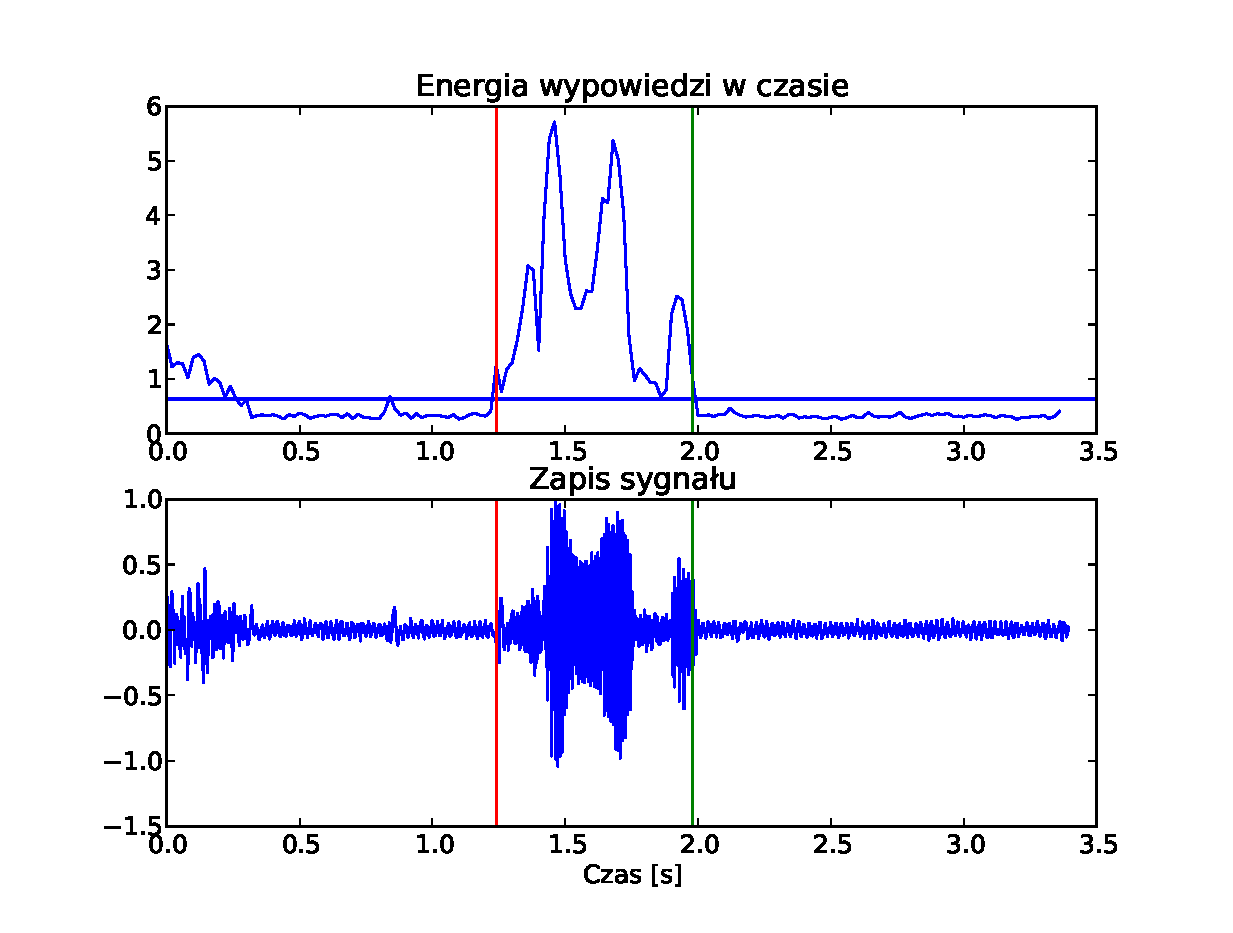
\includegraphics[width=\textwidth]{say_samochod}
    \caption{Energia sygnały zapisu wypowiedzi słowa ,,samochód'' wraz z
    lokalizacją początku i końca wypowiedzi.}
    \label{fig:say}
\end{figure}

Do parametryzacji wypowiedzi użyto współczynników kodowania liniowo predykcyjnego.
Rozwiązanie to jest proste: nie wymaga dużo czasu ani pamięci na obliczenia, a
daje stosunkowo bardzo dobre rezultaty.

Zmotała zaprojektowana sieć feed-forward posiadająca 13 neuronów wejściowych
(odpowiadające ilości współczynników LPC), 19 neuronów warstwy ukrytej oraz 6
neuronów warstwy wyjściowej, co odpowiada ilości osób w bazie. Na rysunku
\ref{fig:network} pokazano schemat połączeń sieci.

\begin{figure}
    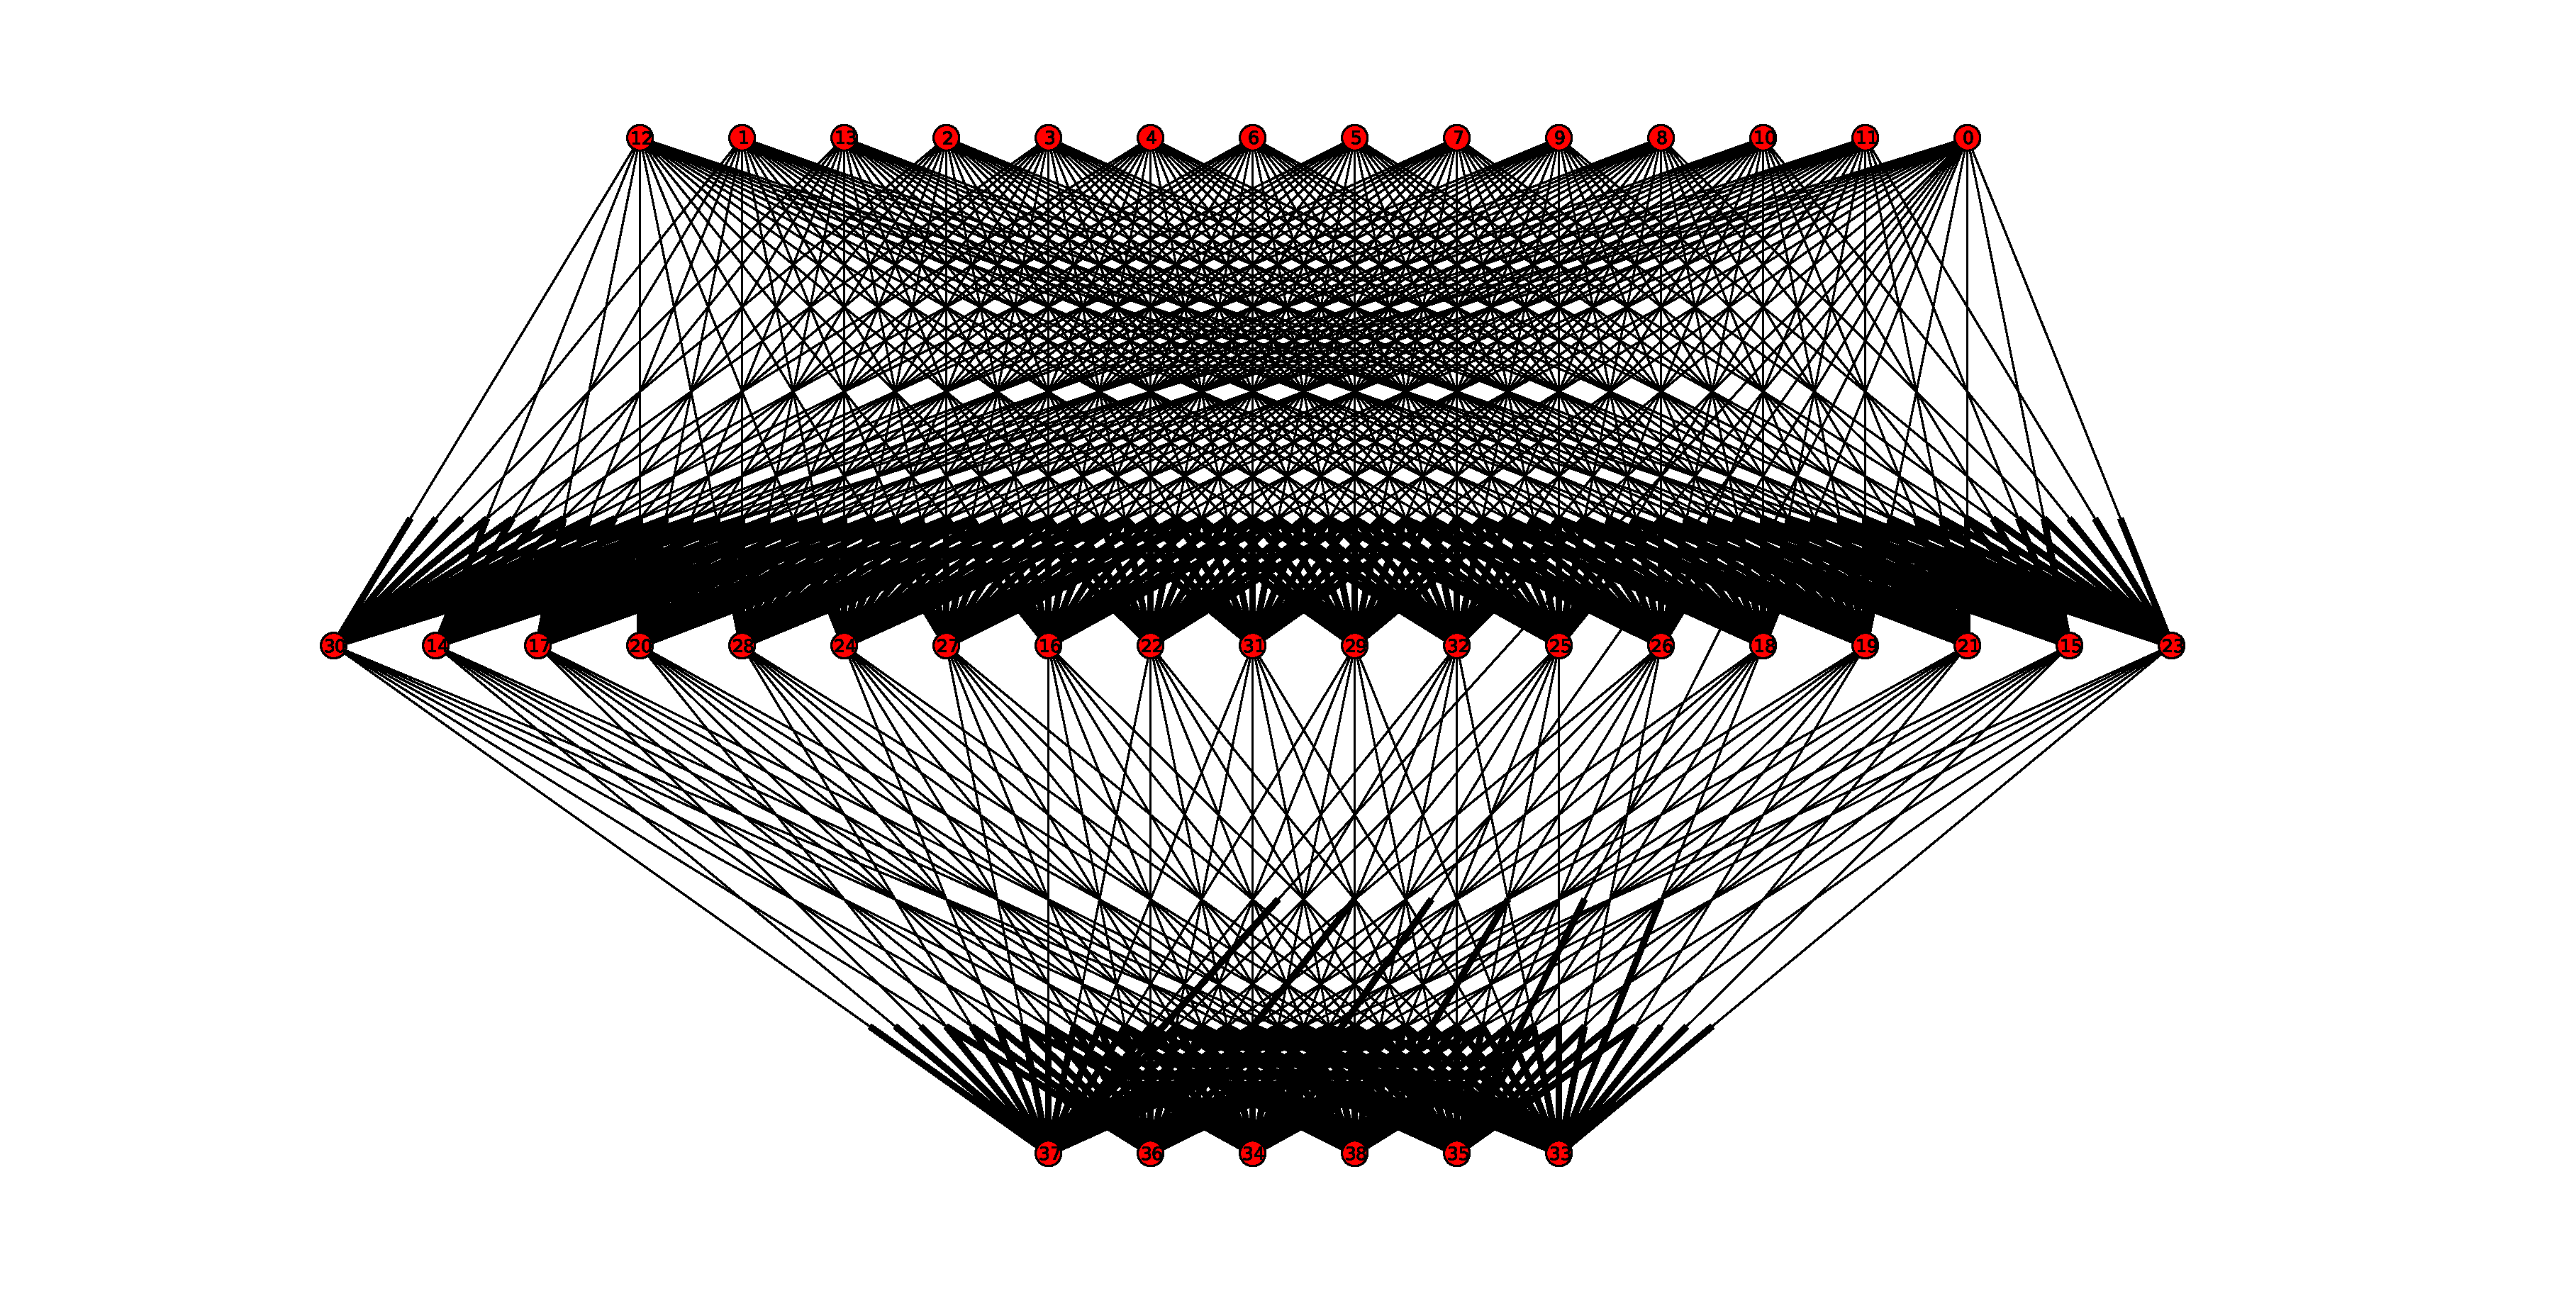
\includegraphics[width=\textwidth]{network}
    \caption{Schemat połączeń sieci neuronowej}
    \label{fig:network}
\end{figure}

\section{Parametryzacja wypowiedzi - ekstrakcja cech}

Jak zostało wcześniej powiedziane cechy wypowiedzi muszą być zależne do
konkretnych osób (wysokość głosu, lokalizacja formantów). Poniżej zostanie
przedstawione kilka sposób estymacji tych wartości z cyfrowych próbek mowy.

\textbf{Dyskretna Transformata Fouriera} - w przeciwieństwie do sygnału w
dziedzinie czasu, w dziedzinie częstotliwości można uzyskać informacje o tonie
głosu i lokalizacji formantów. Jednak transformata Fouriera zawiera zbyt dużo
niepotrzebnych informacji, co bardzo utrudnia jej użycie w przypadku
zastosowania sieci neuronowych.

\textbf{Linear Predictive Coding, LPC} - kodowanie liniowo predykcyjne to
prosta, a zarazem potężna metoda wyciągania informacji o lokalizacji formantów.
W skrócie algorytm LPC pozwala znaleźć wektor współczynników opisujących
widmową obwiednię amplitudy DFT. Współczynniki każdej próbki mogą być wyliczone
jako liniowa kombinacja współczynników próbki poprzedniej, co pokazuje równanie
\ref{eqn:lpc}.

\begin{equation}\label{eqn:lpc}
    x(n) - \sum_{k=1}^p a_k x(n-k) + e(n)
\end{equation}

$p$ współczynników $a_k$ minimalizujących błąd między sygnałem a jego estymatą
są znane jako współczynniki LPC $p$-tego rzędu. Współczynniki LPC 13-rzędu dla
słowa ,,samochód'' dla wszystkich osób z bazy znajdują się na rysunku
\ref{fig:lpc}.

\begin{figure}
    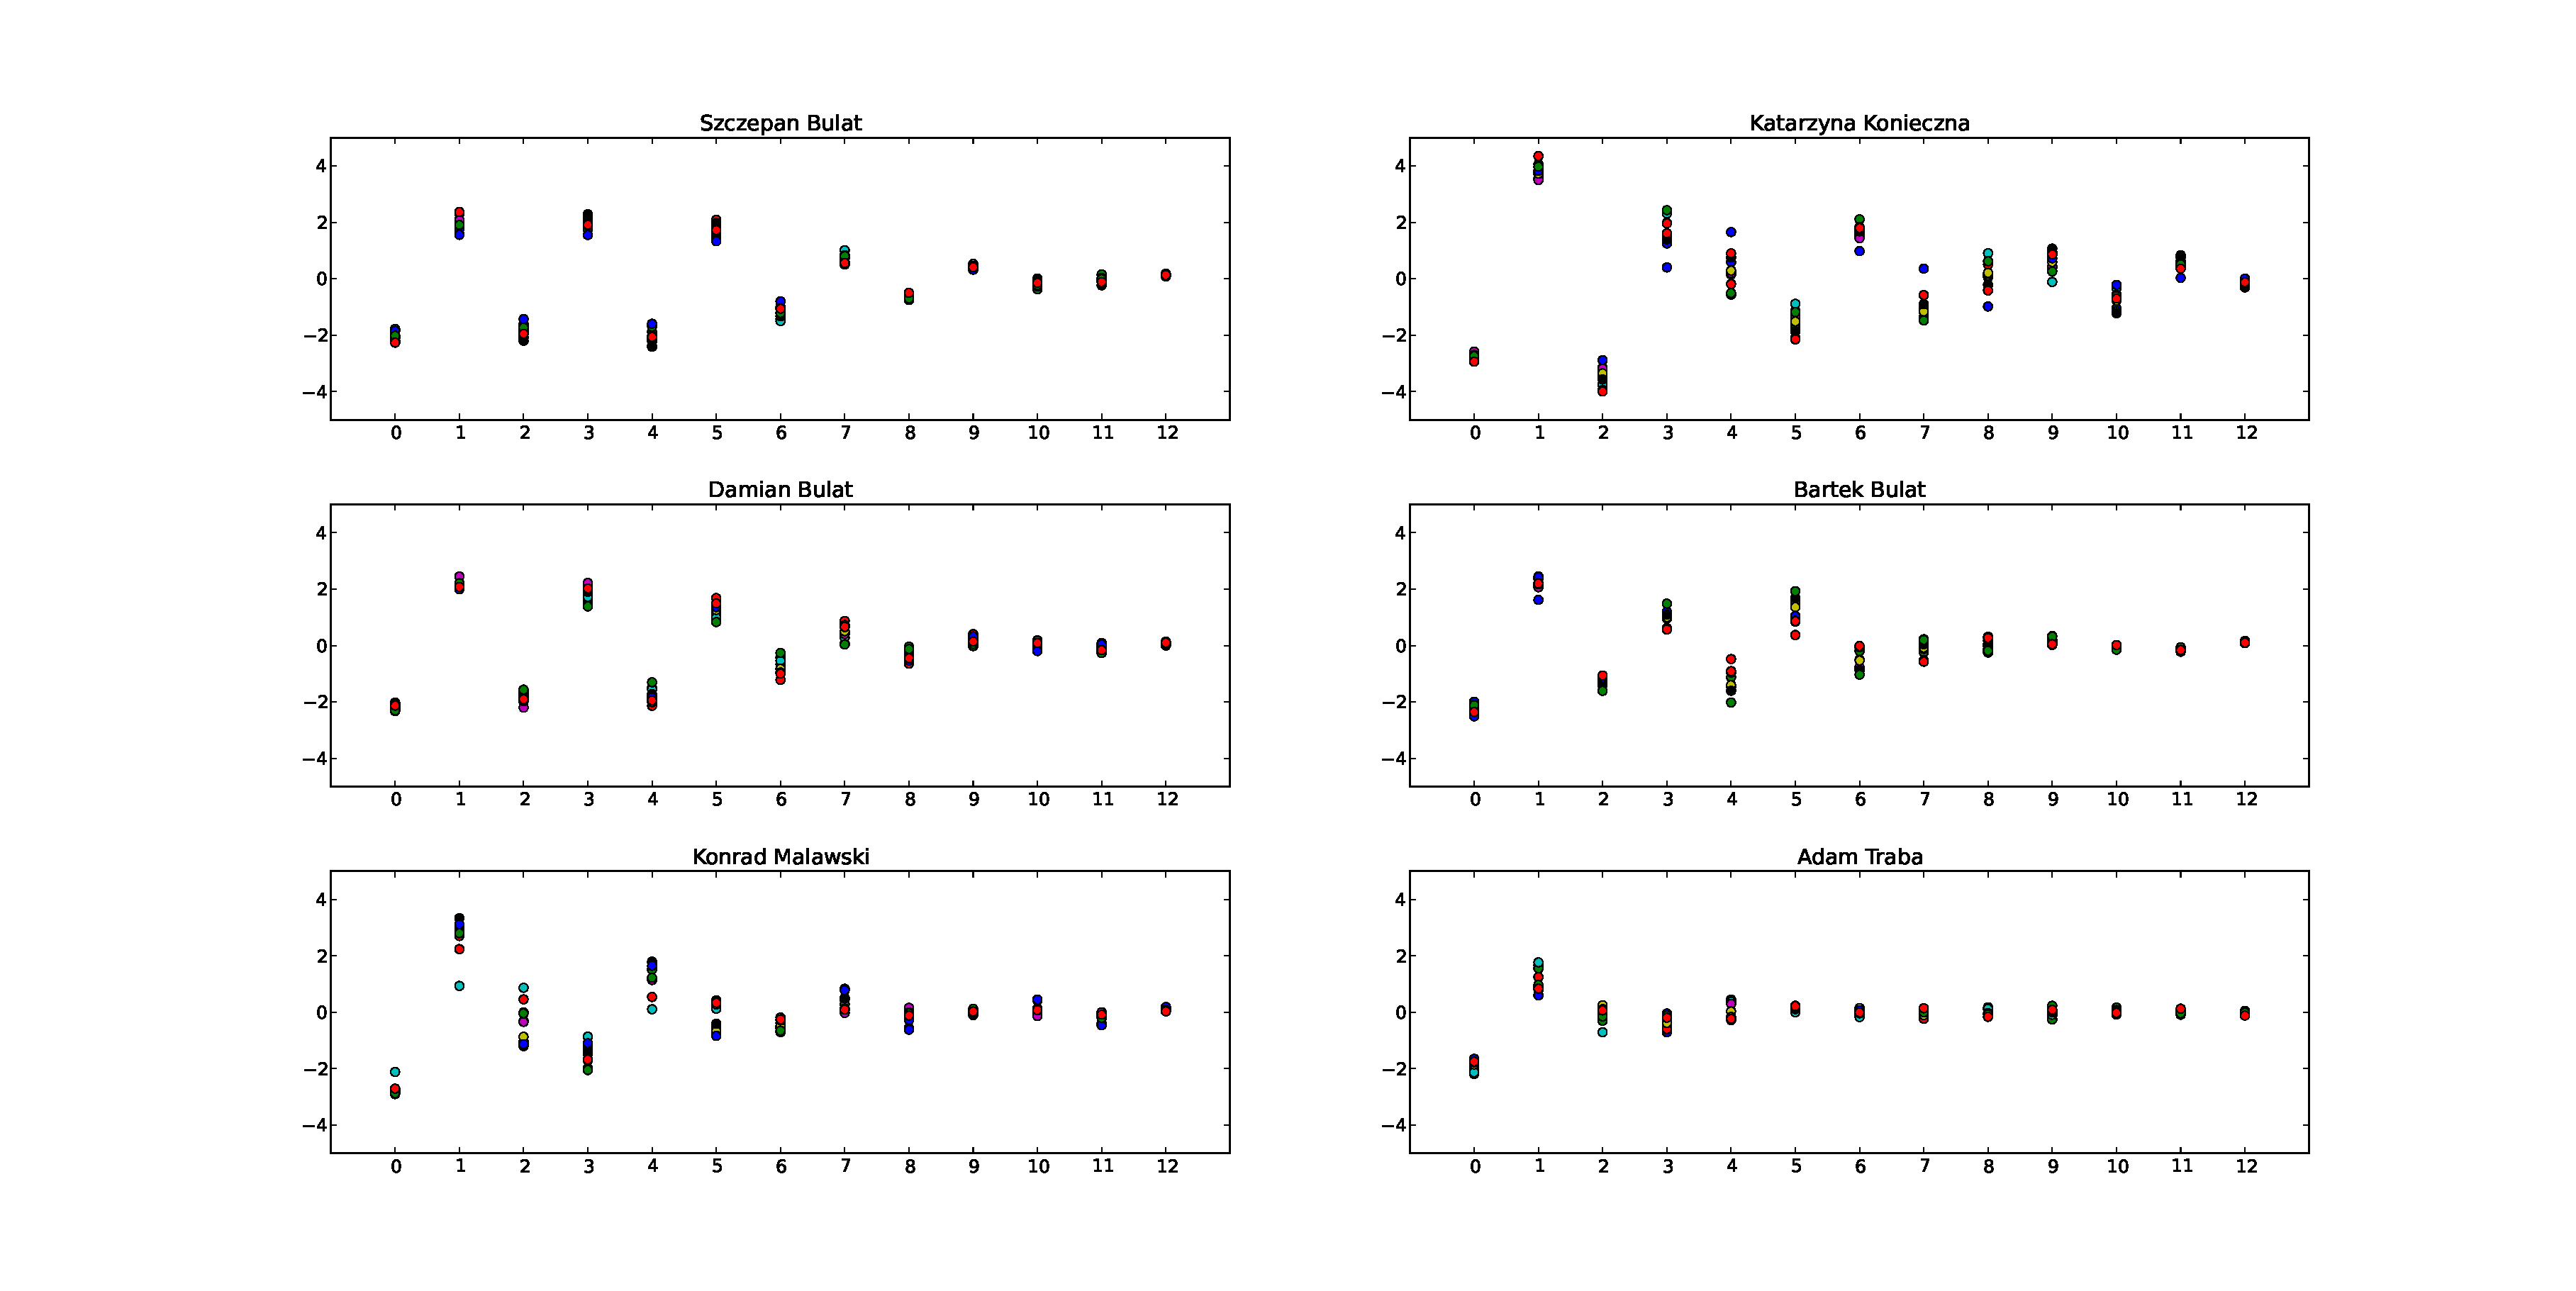
\includegraphics[width=\textwidth]{lpc_samochod}
    \caption{Współczynniki LPC 13-tego rzędy dla wszystkich osób z bazy}
    \label{fig:lpc}
\end{figure}

\textbf{Współczynniki Cepstralne} - te współczynniki niosą bardzo podobne
informacje jak współczynniki LPC. Opisują obwiednie widmową amplitudy DFT.
Cepstrum to transformata Fouriera z logarytmu amplitudy transformaty Fouriera
sygnału (patrz równanie \ref{eqn:cepstrum}).

\begin{equation}\label{eqn:cepstrum}
    C = DFT( \log ( | DFT (x) | ) )
\end{equation}

Cepstrum zmniejsza liniowy trend spectrum oraz usuwa z sygnału informacje o
mówcy, ta strata informacji przydatna jest w aplikacjach do rozpoznawania
treści wypowiedzi.

Współczynniki cepstralne można obliczyć z współczynników LPC z użyciem
zależności \ref{eqn:lpc_cep}.

\begin{equation}\label{eqn:lpc_cep}
    c_i = a_i + \frac{1}{i} \sum_{j=1}^{i-1} (j)a_{i-j} c_j
\end{equation}

Użycie współczynników cepstralnych, oprócz tego, że usuwa informacje o mówcy i
daje się wyliczyć z LPC nie przyniosło poprawy rezultatów rozpoznawania,
dlatego do dalszej analizy wybrano współczynniki LPC 13-tego rzędu.


\section{Budowa sieci neuronowej}

Sieć nieuronowa użyta w badaniach to typowa, trzywarstwowa sieć neuronowa
feed-forward. Głównym problemem przy projektowaniu sieć do rozpoznawania mówców
jest to, że ilość rozpoznawanych osób musi być znana na początku. Ilość
neuronów warstwie wyjściowej odpowiada rozmiarowi bazy osób, a aktywacja
wyjścia jest tożsama z rozpoznaniem danej osoby.

Ilość neuronów w warstwie wejściowej odpowiada ilości współczynników LPC, czyli
13. Jak można zaobserwować na rysunku \ref{fig:lpc} wyższy rząd współczynników
nie poprawił by rezultatów, bo dla każdej z osób te współczynniki są bardzo
bliskie zeru.

Ilość neuronów w warstwie ukrytej jest dobrana doświadczalnie. Dla mniejszej
liczby sieć miała problemy z zapamiętywaniem wzorców, a dla większej liczby nie
było widocznej poprawy rezultatów.

\section{Testowanie}

W czasie testów skupiono się na dwóch ważnych aspektach tego problemu.
Rozpoznawanie zależne/niezależne od treści słowa oraz sposób uczenia sieci
neuronowej.

\subsection{Zależność od treści}

Nasza baza próbek glosuj pozwoliła nam na testy jakości rozpoznawania mówcy w
przypadku użycia tych samych i różnych słów przez każdą osobę. Imię i nazwisko
jest inne dla prawie każdej osoby, a pozostałe dwa słowa (,,samochód'' i
,,kot'') były wypowiedziane przez każdą osobę z bazy. Wykres \ref{fig:word}
przedstawia parametry analizy regresji sieci uczonej metodą wstecznej
propagacji błędu z momentem, dla wszystkich czterech słów.

\begin{figure}[h!]
    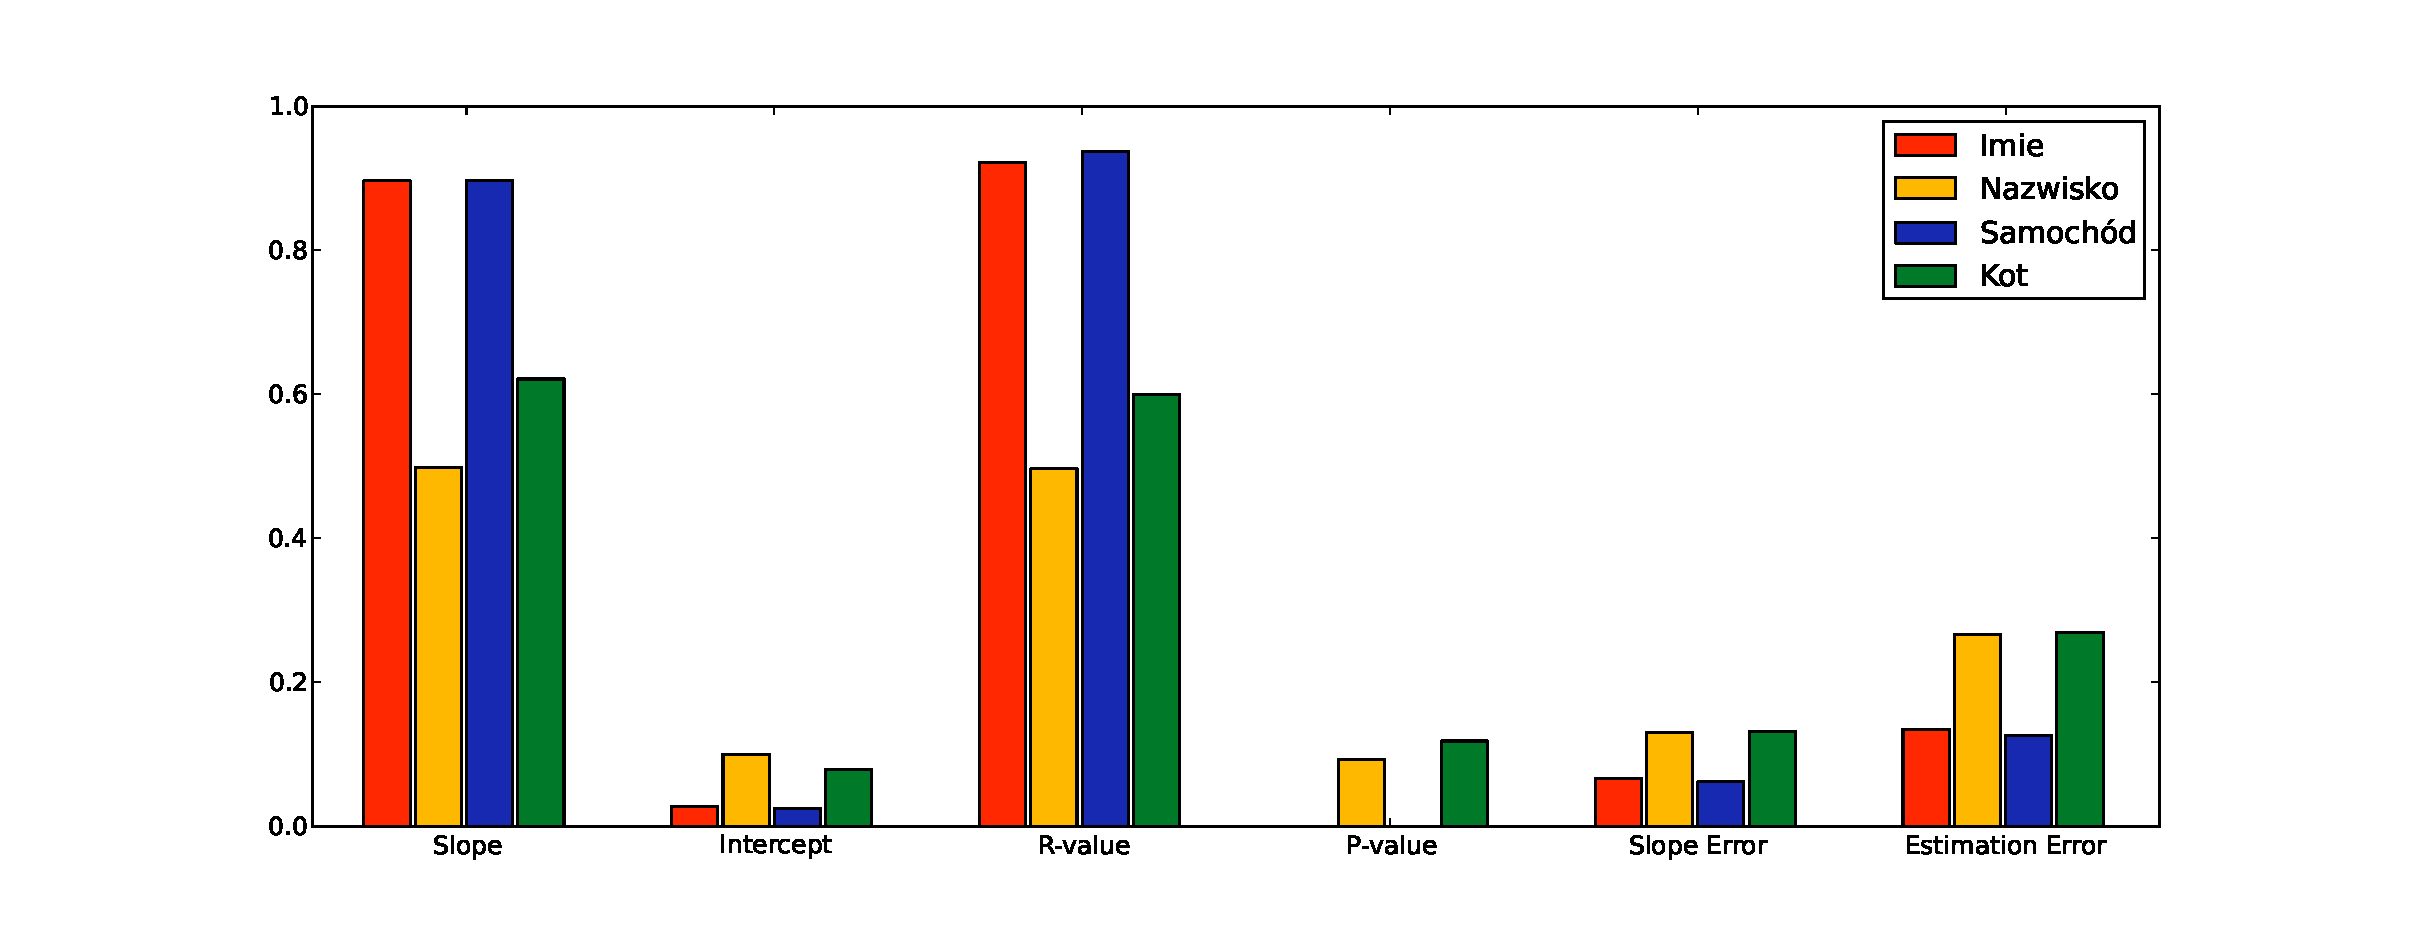
\includegraphics[width=\textwidth]{word_network_reggresion}
    \caption{Wykres parametrów regresji liniowej w zależności od słowa użytego
    do rozpoznawania}
    \label{fig:word}
\end{figure}

Najlepszą metodą (parametry opisującą prostą regresji zbliżone do $y=x$, niski
błąd, wysoka korelacja wyjścia i wejścia) okazała się metoda zależna od treści,
mianowicie wykorzystanie słowa ,,samochód''. Wykorzystanie słowa ,,kot'',
pomimo, że jest to również metoda zależna od treści (która z założenia powinna
dawać lepsze rezultaty), jest metodą najgorszą. Duży wpływ na taki wynik może
mieć to, że słowo ,,kot'' jest bardzo krótkie, co za tym idzie, niesie mało
informacji.

Dobre efekty dało również wykorzystanie imienia osoby jako analizowanego słowa,
wpływ na to może mieć to, że żadne z imion się nie powtarza. Wykorzystanie
nazwiska nie dało zadowalających rezultatów, może to być spowodowane tym, że w
badzie występują 3 osoby o tych samych nazwiskach.

\subsection{Sposób trenowania sieci}

Użyta implementacja trenowanie sieci czterema algorytmami, dodatkowo jeden
algorytm jest zaimplementowany w wersji wielowątkowej (na wiele procesorów).
Dostępne algorytmu uczenia:
\begin{description}
    \item[Alg. wstecznej propagacji błędu z momentem] prosta metoda wstecznej
        propagacji błędu z zachowaniem momentu, co zapobiega na utkwieniu sieci
        w ekstremach lokalnych lub siodłach.
    \item[Alg. RProp] inna metoda wstecznej propagacji błędu.
    \item[Gradient sprzężony] - adaptacja metody numerycznego wyznaczania
        ekstremów dla sieci neuronowych
    \item[Alg. BFGS] - ta metoda jest również zaimplementowana wielowątkowo.

\end{description}
Podobnie jak w przypadku różnych słów przeprowadzono testy regresji liniowej
dla każdego sposobu uczenia. Porównanie parametrów znajduje się na wykresie
\ref{fig:train}.


\begin{figure}[h!]
    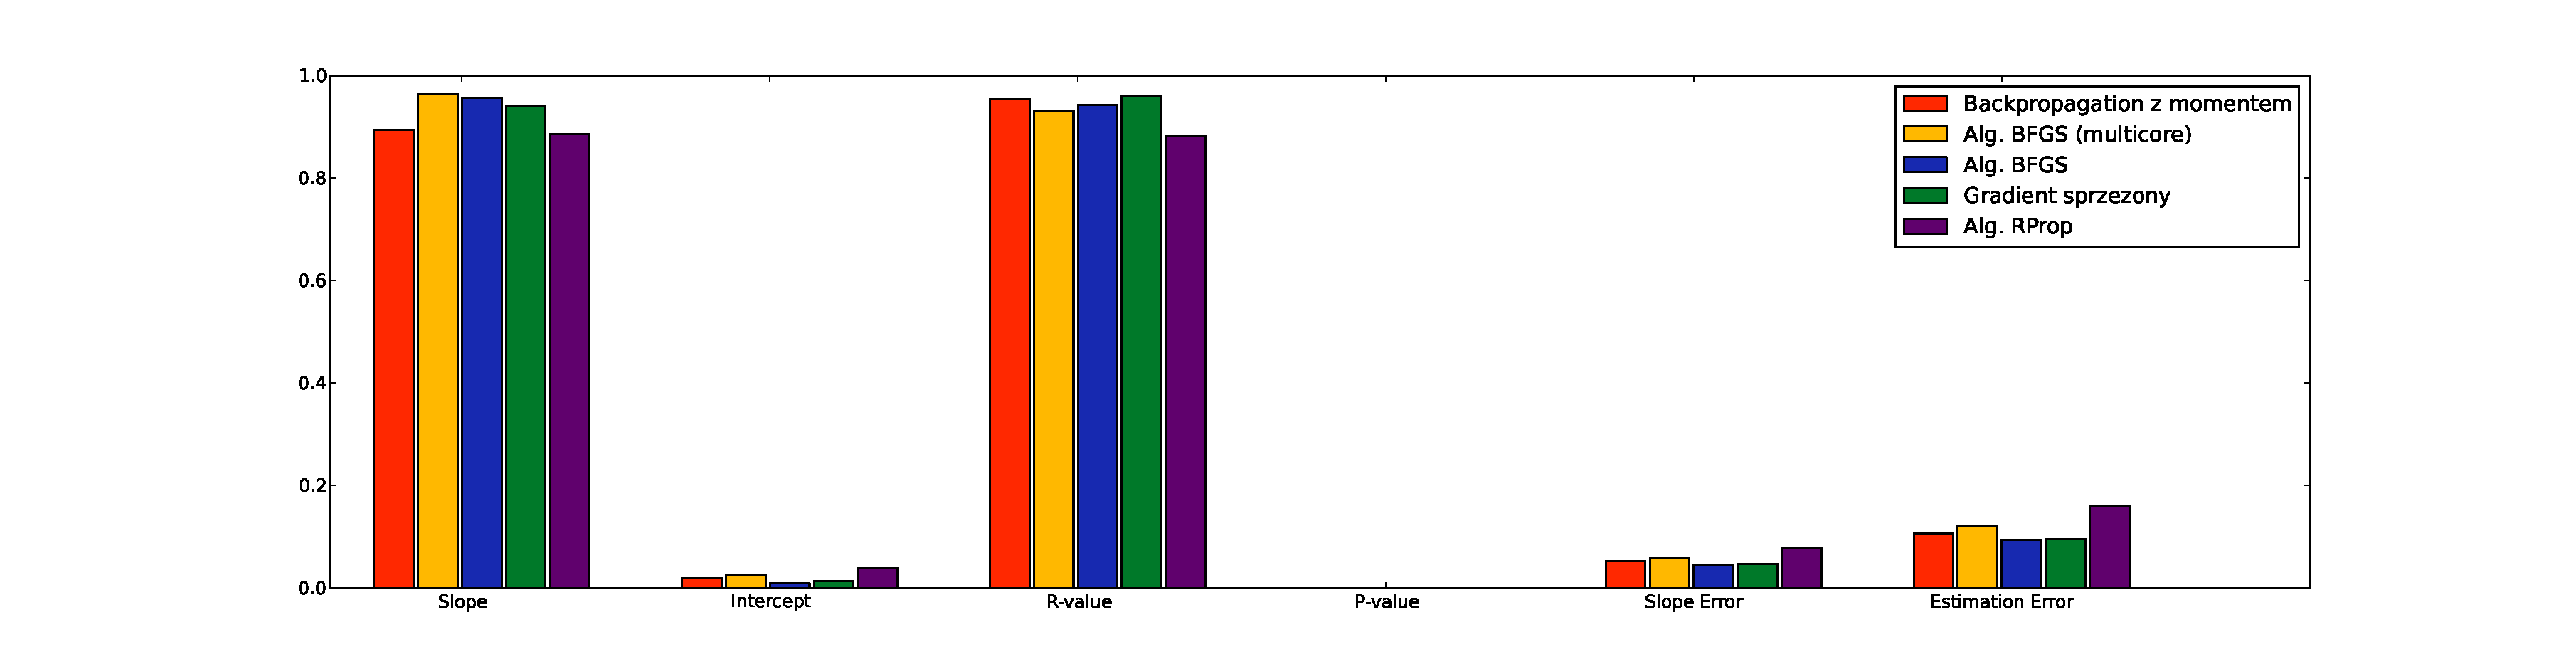
\includegraphics[width=\textwidth]{training_network_reggresion}
    \caption{Wykres parametrów regresji liniowej w zależności od metody uczenia
    sieci neuronowej}
    \label{fig:train}
\end{figure}

Żadna z pokazanych metod uczenia nie wykazała znaczącej przewagi nad innymi.
Można jedynie zauważyć, że metoda wykorzystująca algorytm RProp daje rezultaty
sporo poniżej wartości średniej.

\section{Podsumowanie}

W trakcie badań udało się zaimplementować podany algorytm wykrywania aktywności
mówcy, wyliczanie współczynników LPC. Do zastosowań pozatestowych do uczenia
sieci użyto algorytmu BFGS i wybrano porównanie na podstawie słowa ,,samochód''.

W rozwoju aplikacji zostało kilka miejsc do uzupełnienia, takich jak
znalezienie lepszych parametrów opisujących wypowiedź, takich które przechowują
więcej cech osobowych, czy też sprawdzanie poprawności klasyfikacji z użyciem
większej ilość długich słów.

\section{Bibliografia}
\begin{thebibliography}{123}
    \bibitem{textind}Text-Independent Speaker Recognition Based on Neural Networks,
        \url{http://www.neuralnetworks.it/neuralnetspeaker.asp}
    \bibitem{VINING}Automatic Speaker Recognition Using Neural Networks, \emph{Braian
        J. Love, Jennifer Vining, Xuening Sun}, 2004
    \bibitem{FFNET}Fast-forward neural network library for python,
        \url{http://ffnet.sourceforge.net/}
    \bibitem{github}Repozytorium zawierające kod źródłowy omawianego projektu,
        \url{https://github.com/barthez/speaker-recognition-nn}
\end{thebibliography}

\section{Dodatek A: Opis aplikacji}

Zostało przygotowanych kilka skryptów które realizują wszystkie zadania
dotyczące rozpoznawania mówcy. Głównym skryptem jest \verb|network_test.py|.
Pozwala on na nauczenie sieci (parametr \verb|-a learn|) oraz na próbe
dopasowania wzorca z bazy (\verb|-a test|) lub nagrania i dopasowania nowego
wzorca (\verb|-a record|). Aby określić słowo które ma zostać uzyte w
uczeniu/testowaniu nalezy dodać parametr \verb|-w słowo|.

\end{document}
